\begin{noheadline}

\begin{frame}[allowframebreaks]{Table of Contents}

\tableofcontents

\end{frame}

\end{noheadline}


\section{Introduction}
\subsection{Contacts}
\begin{frame}{Contacts}
    \begin{itemize}
        \item \textbf{Name:} Bruno Taborda
        \item  \textbf{Email:}\href{mailto:Bruno\_Taborda@iscte-iul.pt}{Bruno\_Taborda@iscte-iul.pt}
    \end{itemize}
\end{frame}

\subsection{What is GitHub?}
\begin{frame}{What is GitHub?}
    \begin{itemize}
        \item Open-source repository hosting service (\href{https://github.com/}{https://github.com/});
        \item Hosts your source code in multiple programming languages;
        \item Hosts your documentation;        
    \end{itemize}
    \centering
    
\includegraphics[scale=.3]{github}
\end{frame}

\subsection{Why use Github?}
\begin{frame}{Why use Github?}
\begin{itemize}
    \item Easy to contribute;
    \item Easy documentation;
    \item Keep tracking changes in files;
    \item Variety of integration options (e.g. slack).
    \item Has non-compiled files (e.g. .py) and non-vendor files (e.g. .txt);
\end{itemize}
\end{frame}

\section{Repository}
\subsection{Repository}
\begin{frame}{Repository}
    \begin{itemize}
        \item Used to store the source code and documentation;
        \item Should include a licence file and a README file with the description;
        \item Private repository: Only authorized users can see the repository;
        \item Public repository: Anyone can use see or collaborate with you.      
    \end{itemize}
\end{frame}

\subsection{Issues \& Milestones}
\begin{frame}{Issues \& Milestones}
    \begin{itemize}
        \item Keep track of tasks, enhancements and bugs;
        \item Prioritize your work and know what was done;
        \item Assign issues to contributors;
        \item Comment and review issues;
        \item Use milestones to know the deadline of a issue.
    \end{itemize}
\end{frame}

\subsection{Labels \& Wiki}
\begin{frame}{Labels \& Wiki}
    \begin{itemize}
        \item Labels are important to identify the content of a issue;
        \item Wiki allow us to have a easy documentation available for everyone.
    \end{itemize}
    \centering
    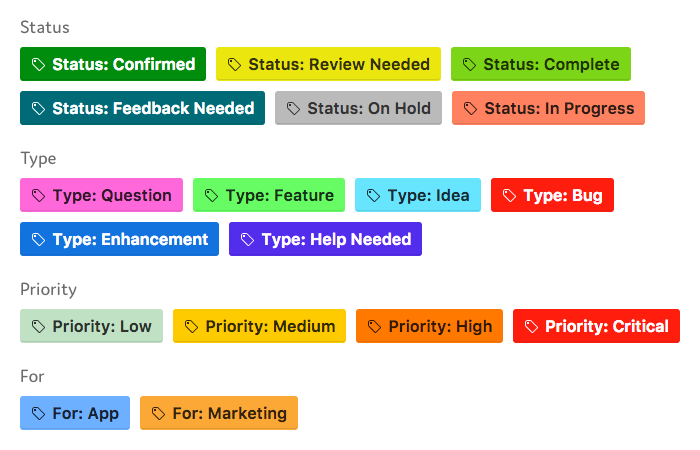
\includegraphics[scale=.3]{github_labels}
\end{frame}

\subsection {Branchs \& Merge}
\begin{frame}{Branchs \& Merge}
    \centering
    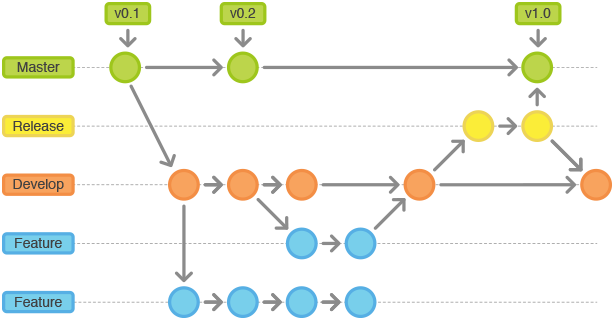
\includegraphics[scale=.5]{github_branch_merge}
\end{frame}

\subsection {Pull request}
\begin{frame}{Pull request}
    \begin{itemize}
        \item Pull requests let you tell others about changes you've pushed to a branch in a repository on GitHub;
        \item You can discuss and review the potential changes with collaborators;
        \item Add follow-up commits before your changes are merged into the base branch.
    \end{itemize}
\end{frame}


\section{Git commands}
\subsection{Git commands}
\begin{frame}{Git commands}
    \begin{itemize}
        \item git config - -global
        \item git clone url
        \item git pull
        \item git add filename or *
        \item git commit -m "message"
        \item git push
        \item git checkout branchname
        \item git merge otherbranchname
    \end{itemize}
\end{frame}

\section{Demo}
\subsection{Demo}
\begin{frame}{Demo}
    \centering
    \href{https://github.com/taborda11/IntroductionGithub}{Introduction to GitHub repository}
    
\end{frame}

